\section{Техническое задание}
\subsection{Основание для разработки}

Основанием для разработки является задание на выпускную квалификационную работу бакалавра "<Веб-приложение для компьютерной поддержки самостоятельной работы  иностранных студентов при изучении языка программирования  JavaScript">.

\subsection{Цель и назначение разработки}

Основной задачей выпускной квалификационной работы является разработка и внедрение веб-приложения для компьютерной поддержки самостоятельной работы  иностранных студентов при изучении языка программирования  JavaScript.

Посредством внедрения веб-приложения планируется устранить существующие недостатки, связанные с неструктурированным доступом к учебным материалам, отсутствием интерактивных инструментов для практики и тестирования, а также сложностями в организации учебного процесса для иностранных студентов, включая языковые барьеры.

Цель разработки включает следующие подцели:

\begin{itemize}
\item создание единой образовательной платформы для доступа к учебным курсам, урокам и тестам;
\item обеспечение удобного и интуитивно понятного интерфейса для самостоятельного изучения JavaScript;
\item интеграция инструментов для проверки знаний, таких как тесты с автоматической оценкой;
\item оптимизация процессов управления учебным контентом для преподавателей и взаимодействия студентов с платформой.
\end{itemize}

\subsection{Функциональные задачи}

Разрабатываемая веб-платформа включает в себя следующие модули:
\begin{enumerate}
\item \textbf{Курсы} — модуль для создания и управления учебными курсами, включающими уроки и тесты. Преподаватели могут добавлять, редактировать и удалять курсы, а студенты получают доступ к материалам.;
\item \textbf{Уроки} — система управления учебным контентом, позволяющая структурировать материалы курса (текст, изображения, видео) и задавать порядок уроков. Поддерживается предпросмотр уроков и их редактирование.;
\item \textbf{Тесты} — модуль для создания и прохождения интерактивных тестов. Преподаватели могут задавать вопросы и варианты ответов, а студенты проходят тесты с автоматической оценкой результатов;
\item \textbf{Результаты тестов} — инструмент для анализа успеваемости студентов. Преподаватели могут просматривать, удалять и управлять результатами тестов, включая статистику по студентам;
\item \textbf{Панель управления преподавателя} — интерфейс для управления курсами, уроками, тестами и результатами, с удобной навигацией и виджетами для быстрого доступа;
\item \textbf{Профиль пользователя} — модуль для управления учетной записью, включая настройки аватара и персональной информации;
\item \textbf{Сообщения} — система уведомлений для обратной связи (например, сообщения об успешном добавлении урока или удалении результатов);
\item \textbf{Панель управления} — страница с виджетами всех вышеперечисленных сервисов.
\end{enumerate}

\subsection{Требования пользователя к интерфейсу web-сайта}

Платформа должна обеспечивать:
\begin{itemize}
    \item авторизацию;
    \item интуитивно понятную навигацию между модулями;
    \item адаптивный интерфейс для десктопных и мобильных устройств.
\end{itemize}

Композиция интерфейса пользователя представлена на рисунках ~\ref{templ:image1}, ~\ref{templ:image2}, ~\ref{templ:image3}, ~\ref{templ:image4}, ~\ref{templ:image5}, ~\ref{templ:image6}, ~\ref{templ:image7}, ~\ref{templ:image8}, ~\ref{templ:image9},  ~\ref{templ:image10}.
\newpage  

Композиция шаблона курсы представлена на рисунке ~\ref{templ:image1} и состоит из:

\begin{itemize}
	\item кнопка для просмотра курса (1);
	\item окна с информацией роли профиля и имени (2);
	\item кнопка для создания курса (3);
	\item кнопка для просмотра своих курсов (4);
	\item кнопка для выхода (5);
	\item кнопка для смены языка (6).
\end{itemize}

\begin{figure}[h]
	\centering
	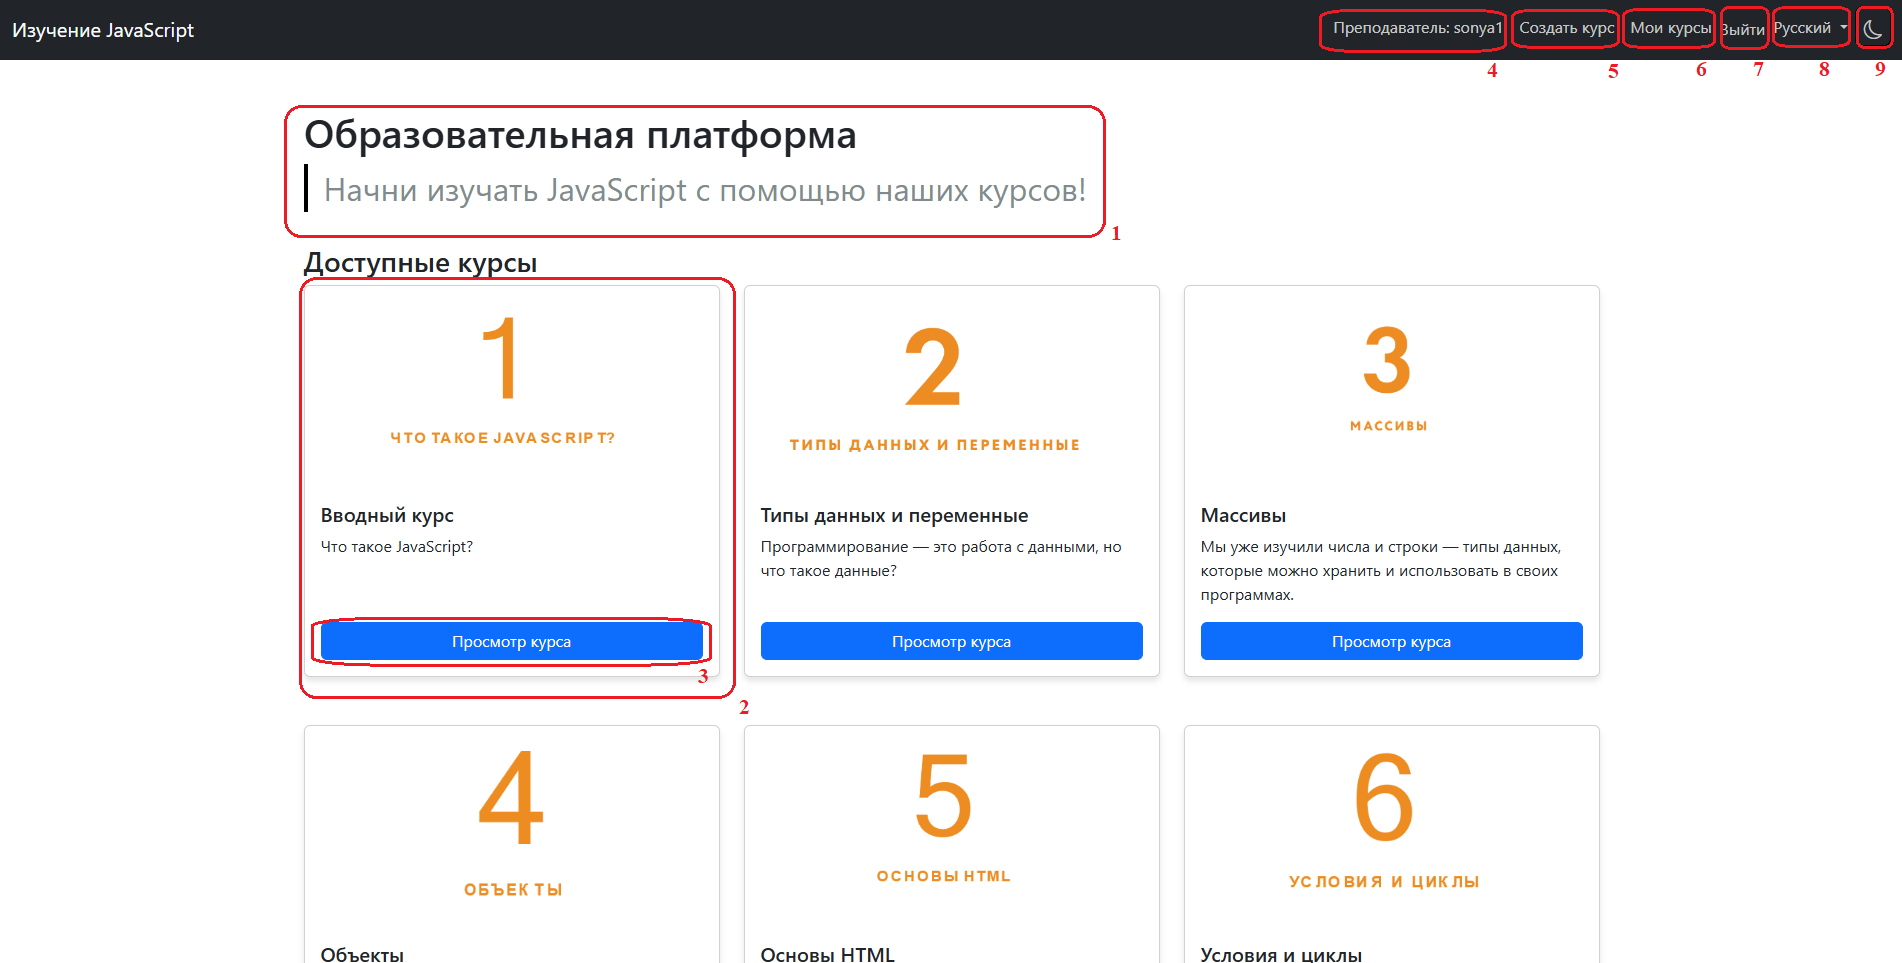
\includegraphics[width=1\linewidth]{images/курсы}
	\caption{Композиция интерфейса сервиса <<Курсы>>}
	\label{templ:image1}
\end{figure}

Композиция шаблона панель управления преподавателя представлена на рисунке ~\ref{templ:image2} и состоит из:

\begin{itemize}
	\item кнопка для редактирования курса (1);
	\item кнопка для управления уроками (2);
	\item кнопка для просмотра курса (3);
	\item кнопка для удаления курса (4).
\end{itemize}

\begin{figure}[h]
	\centering
	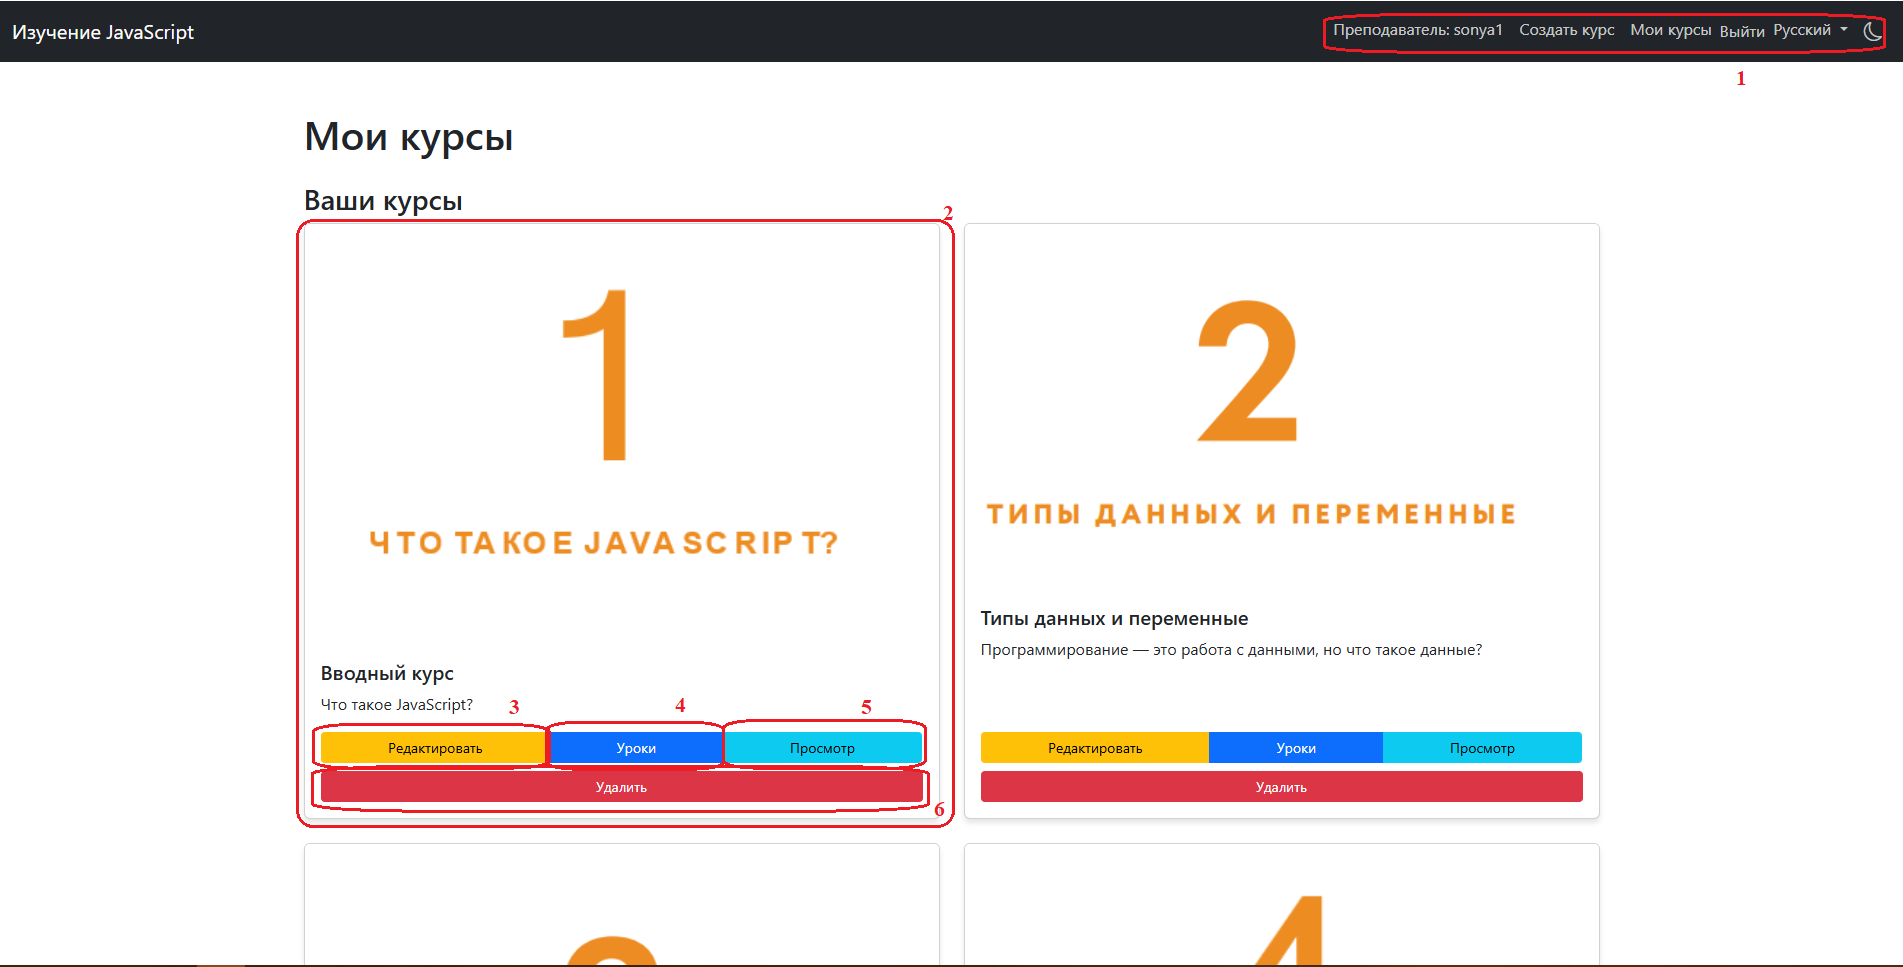
\includegraphics[width=1\linewidth]{images/учитель}
	\caption{Композиция интерфейса сервиса <<Панель управления преподавателя>>}
	\label{templ:image2}
\end{figure}
\newpage 

Композиция шаблона уроки представлена на рисунке ~\ref{templ:image3} и состоит из:

\begin{itemize}
	\item кнопка для просмотра урока (1);
	\item окна курса (2);
	\item окно уроков (3);
	\item навигационная панель (4).
\end{itemize}

\begin{figure}[h]
	\centering
	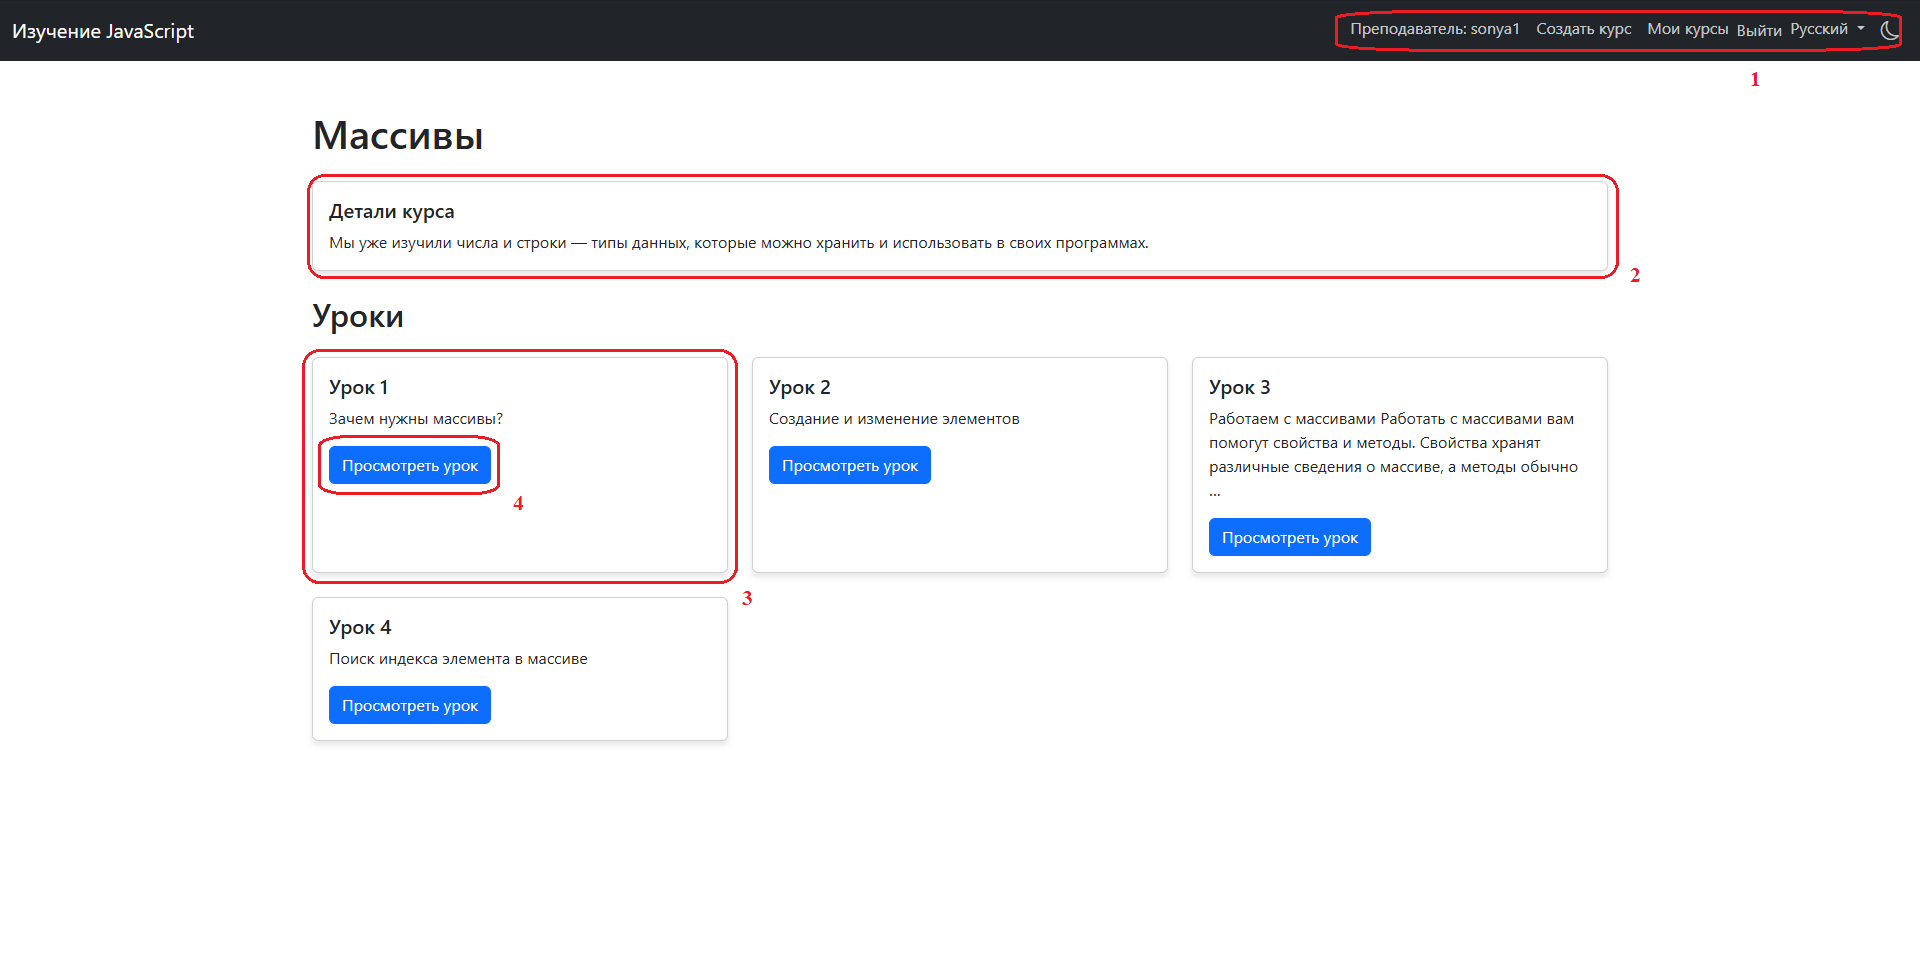
\includegraphics[width=1\linewidth]{images/уроки}
	\caption{Композиция интерфейса сервиса <<Уроки>>}
	\label{templ:image3}
\end{figure}

Композиция шаблона тесты представлена на рисунке ~\ref{templ:image4} и состоит из:

\begin{itemize}
	\item окно уроков (1);
	\item кнопка редактировать урок (2);
	\item кнопка просмотр урока (3);
	\item кнопка обложка урока (4);
	\item кнопка добавить тест (5);
	\item кнопка управление вопросами (6);
	\item кнопка управление результатами (7).
\end{itemize}

\begin{figure}[h]
	\centering
	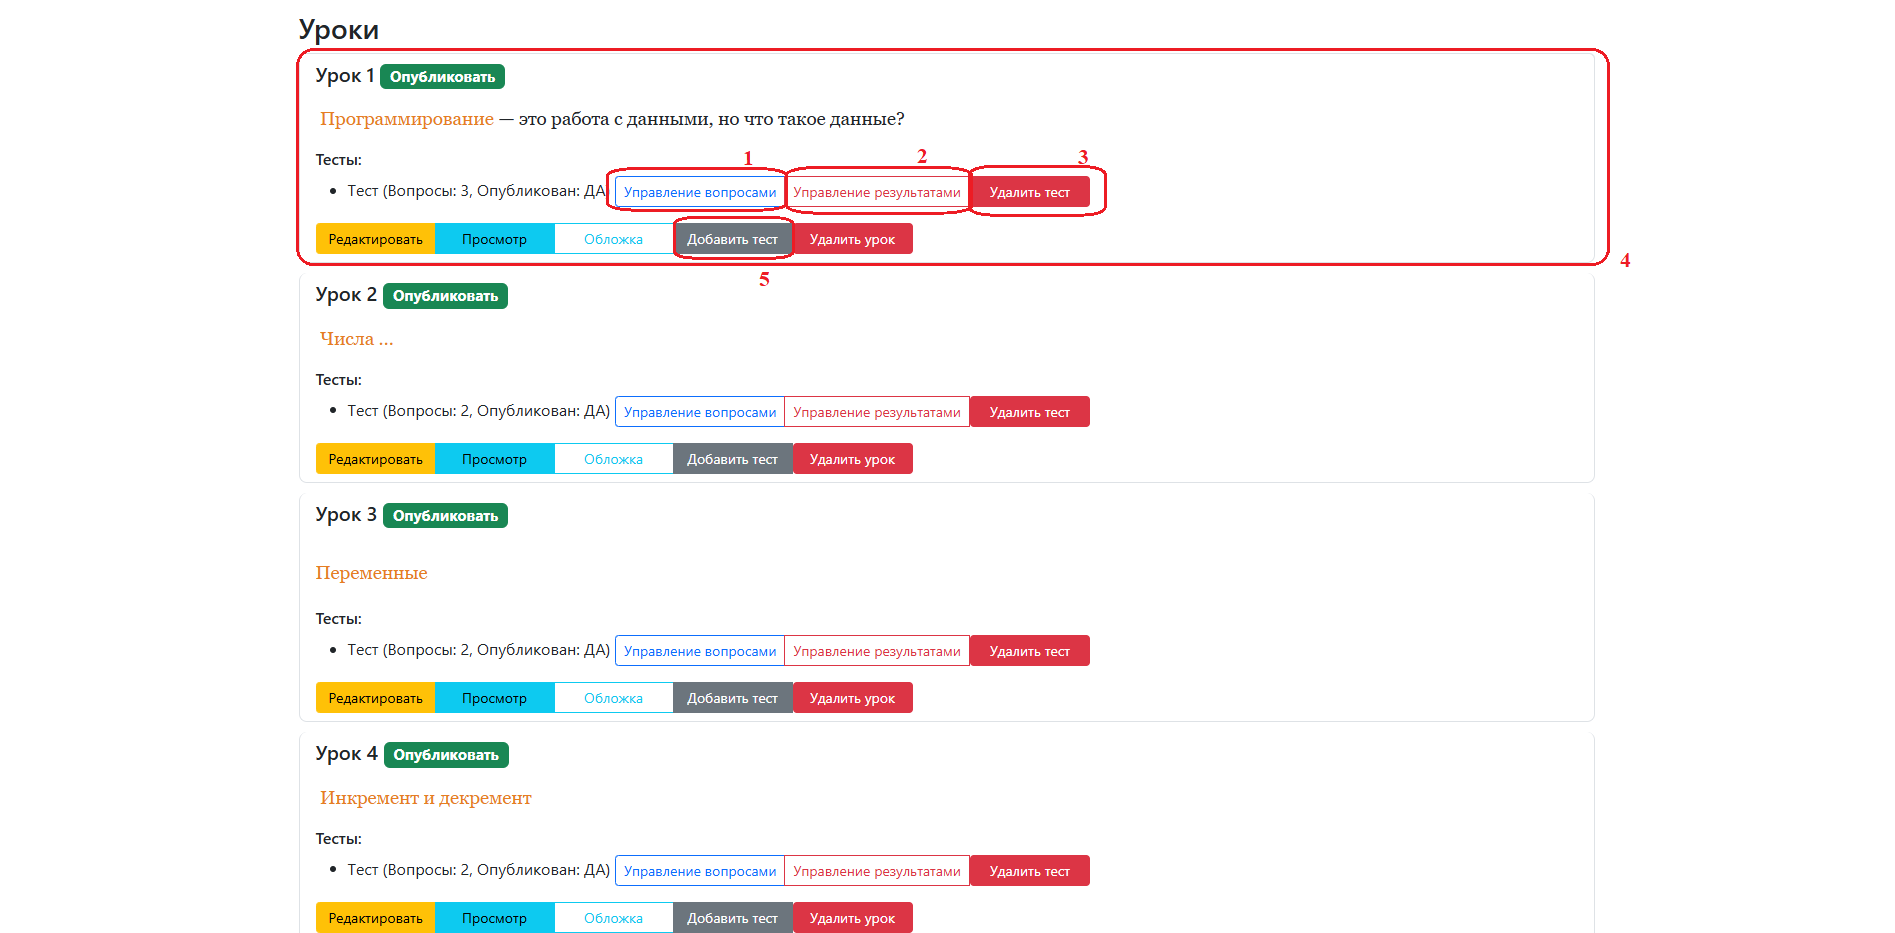
\includegraphics[width=1\linewidth]{images/Тесты}
	\caption{Композиция интерфейса сервиса <<Тесты>>}
	\label{templ:image4}
\end{figure}

Композиция шаблона создание теста представлена на рисунке ~\ref{templ:image5} и состоит из:

\begin{itemize}
	\item окно создания теста (1);
	\item поле ввода заголовка теста (2);
	\item поле ввода описания теста (3);
	\item поле ввода минимального балла (4);
	\item поле выбора статуса (5);
	\item кнопка для создания теста (6);
	\item кнопка возвращения к уроку (7).
\end{itemize}

\begin{figure}[h]
	\centering
	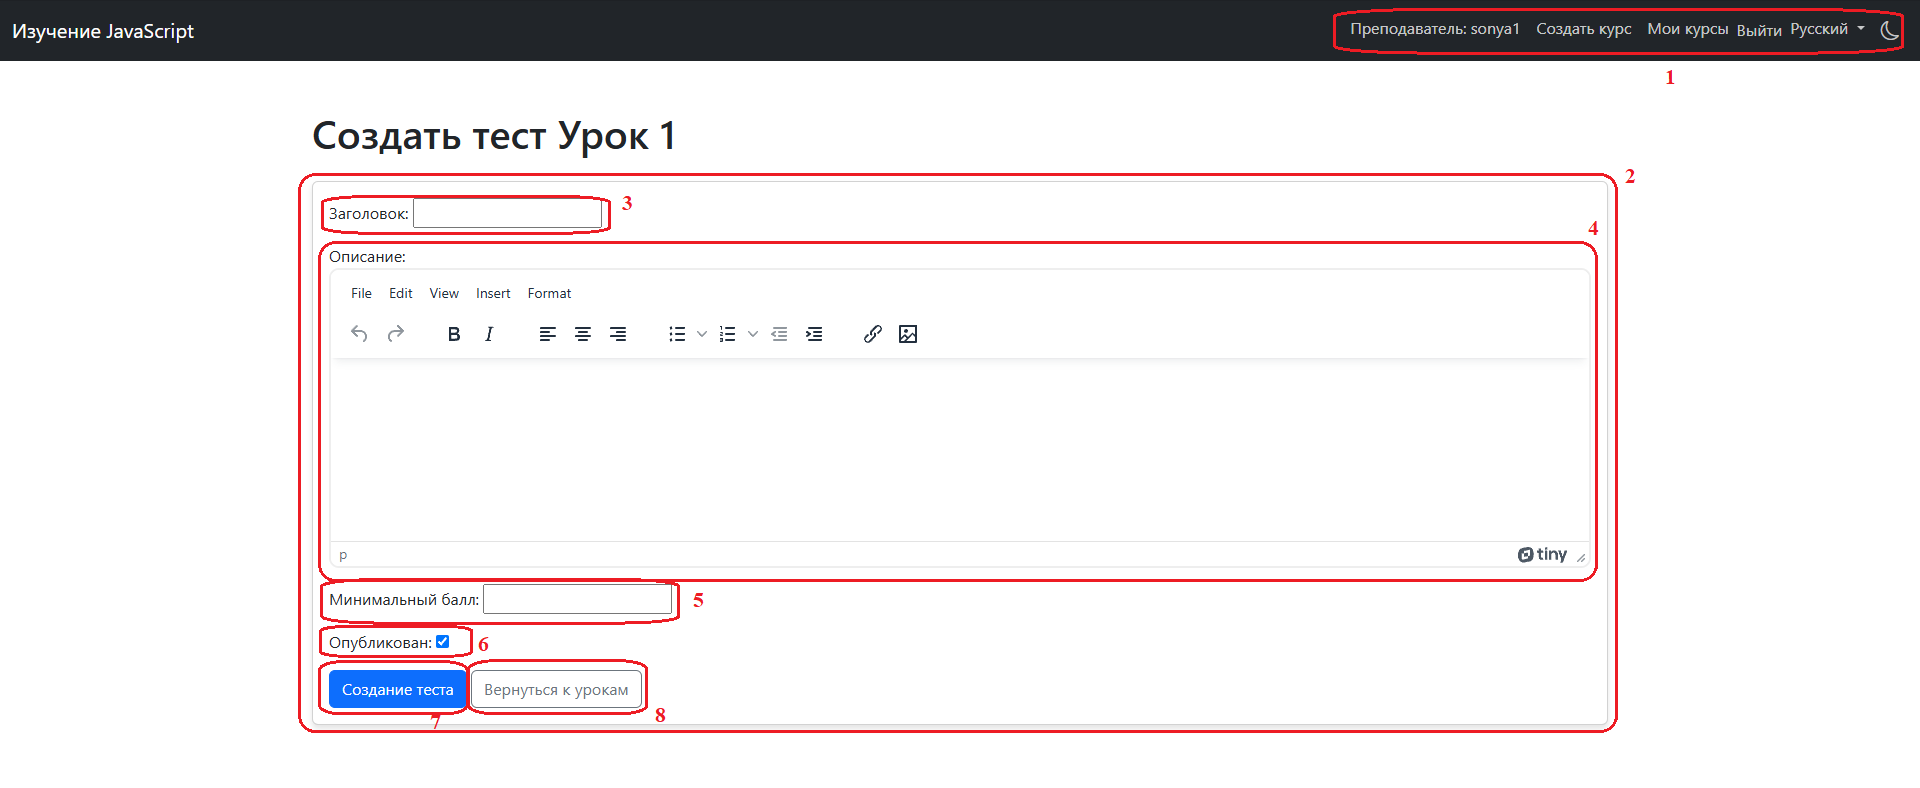
\includegraphics[width=1\linewidth]{images/создатьтест}
	\caption{Композиция интерфейса сервиса <<Создание теста>>}
	\label{templ:image5}
\end{figure}
\newpage

Композиция шаблона результаты теста представлена на рисунке ~\ref{templ:image6} и состоит из:

\begin{itemize}
	\item окна управления результатами теста (1);
	\item окна с результатами студентов  (2);
	\item кнопка удалить все результаты (3);
	\item кнопка удалить результат (4);
	\item кнопка вернуться к вопросам (5);
	\item кнопка вернуться к урокам (6).
\end{itemize}

\begin{figure}[h]
	\centering
	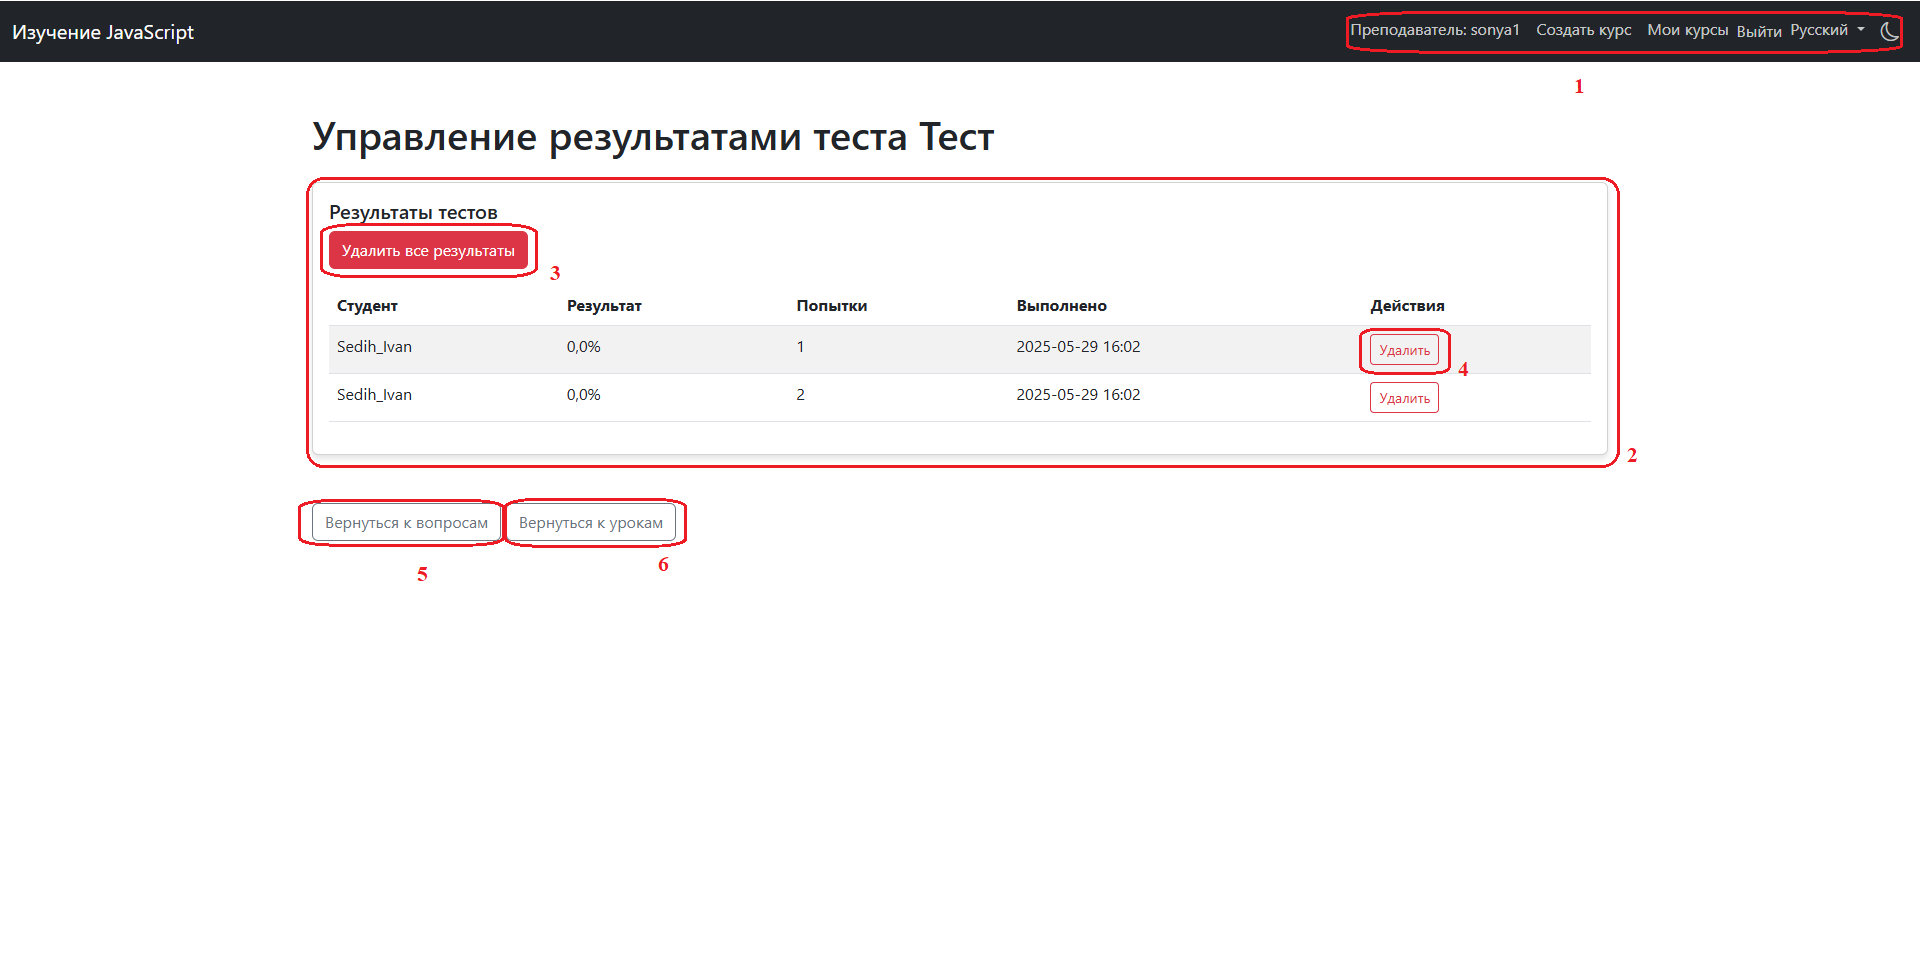
\includegraphics[width=1\linewidth]{images/результаты}
	\caption{Композиция интерфейса сервиса <<Результаты тестов>>}
	\label{templ:image6}
\end{figure}
\newpage
Композиция шаблона окна авторизации представлена на рисунке ~\ref{templ:image7} и состоит из:

\begin{itemize}
	\item поле для ввода кода (1);
	\item экранная клавиатура (2);
	\item кнопка для очистки поля (3);
	\item кнопка для подтверждения ввода пароля (4).
\end{itemize}

\begin{figure}[h]
	\centering
	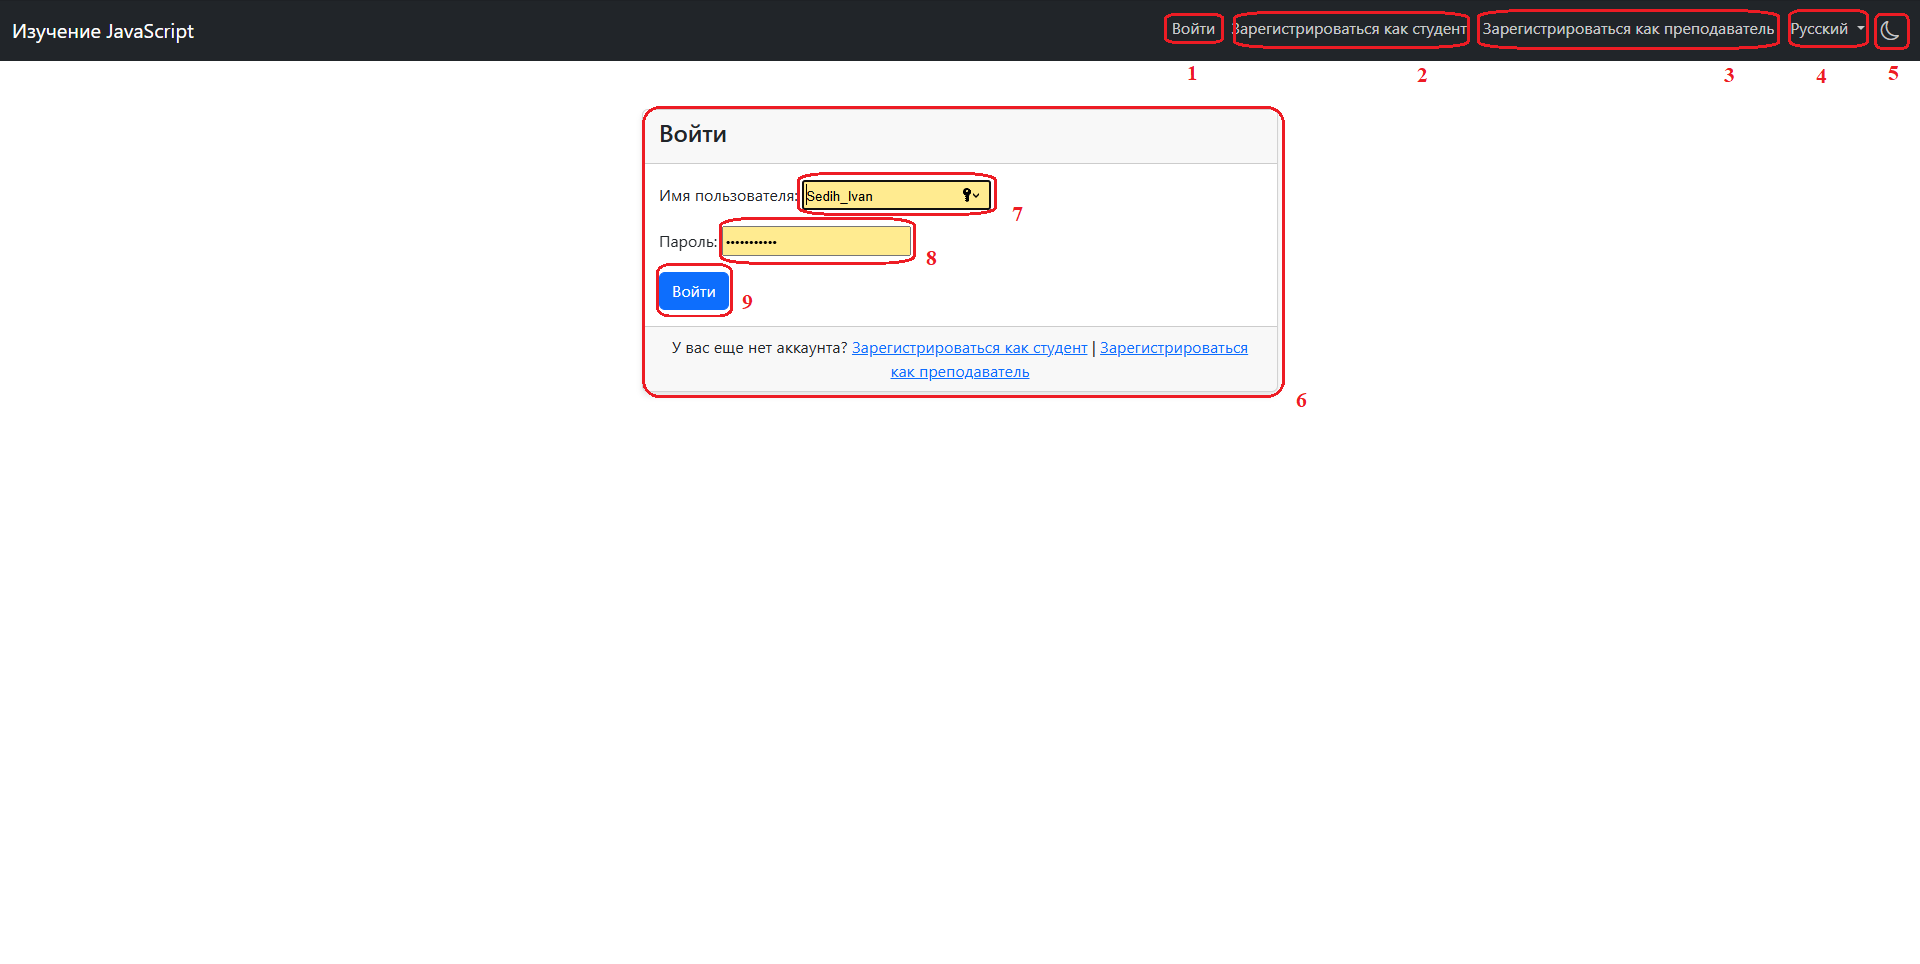
\includegraphics[width=1\linewidth]{images/Авторизация}
	\caption{Композиция интерфейса сервиса <<Авторизация>>}
	\label{templ:image7}
\end{figure}

Композиция шаблона профиль представлена на рисунке ~\ref{templ:image8} и состоит из:

\begin{itemize}
	\item окно курсов на которые записан (1);
	\item кнопка просмотра курса (2);
	\item кнопка отписаться (3).
\end{itemize}

\begin{figure}[h]
	\centering
	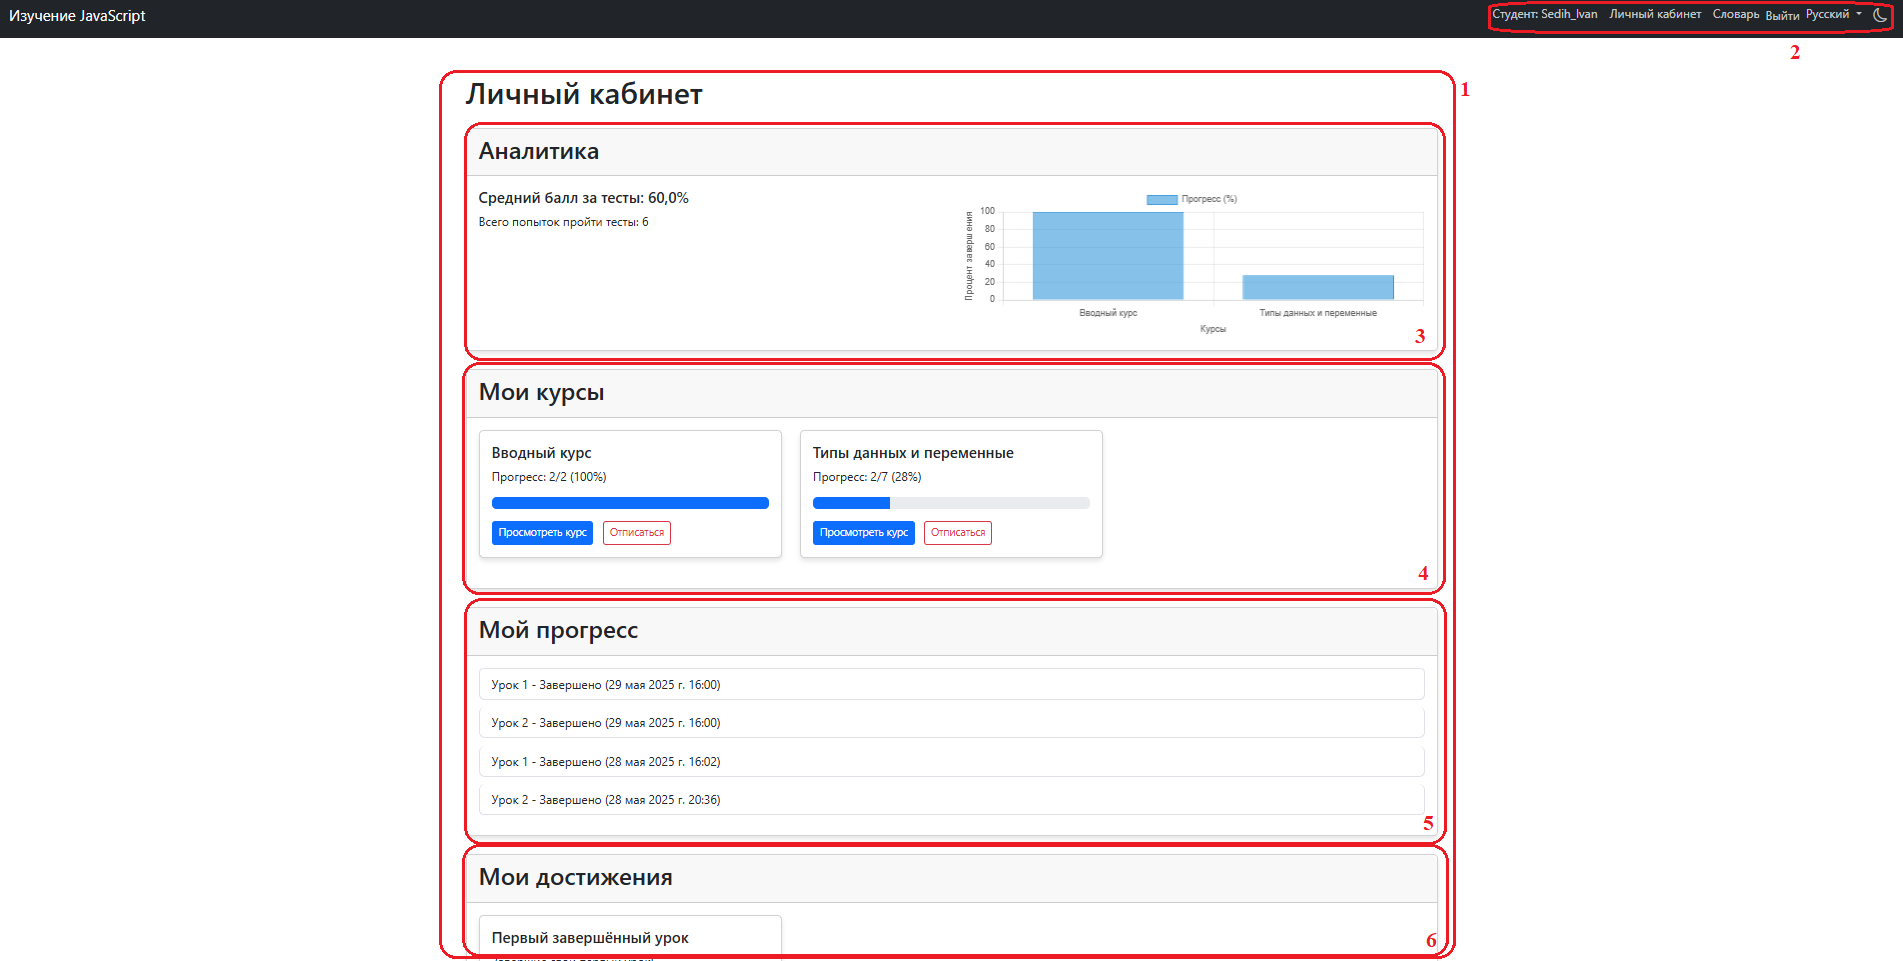
\includegraphics[width=1\linewidth]{images/профиль}
	\caption{Композиция интерфейса сервиса <<Профиль>>}
	\label{templ:image8}
\end{figure}
\newpage

Композиция шаблона создание курса представлена на рисунке ~\ref{templ:image9} и состоит из:

\begin{itemize}
	\item окно создания курса (1);
	\item поле ввода заголовка курса (2);
	\item поле ввода описания курса (3);
	\item кнопка выбора изображения (4);
	\item поле выбора статуса курса (5);
	\item кнопка сохранения курса (6);
	\item кнопка отмены создания курса (7).
\end{itemize}

\begin{figure}[h]
	\centering
	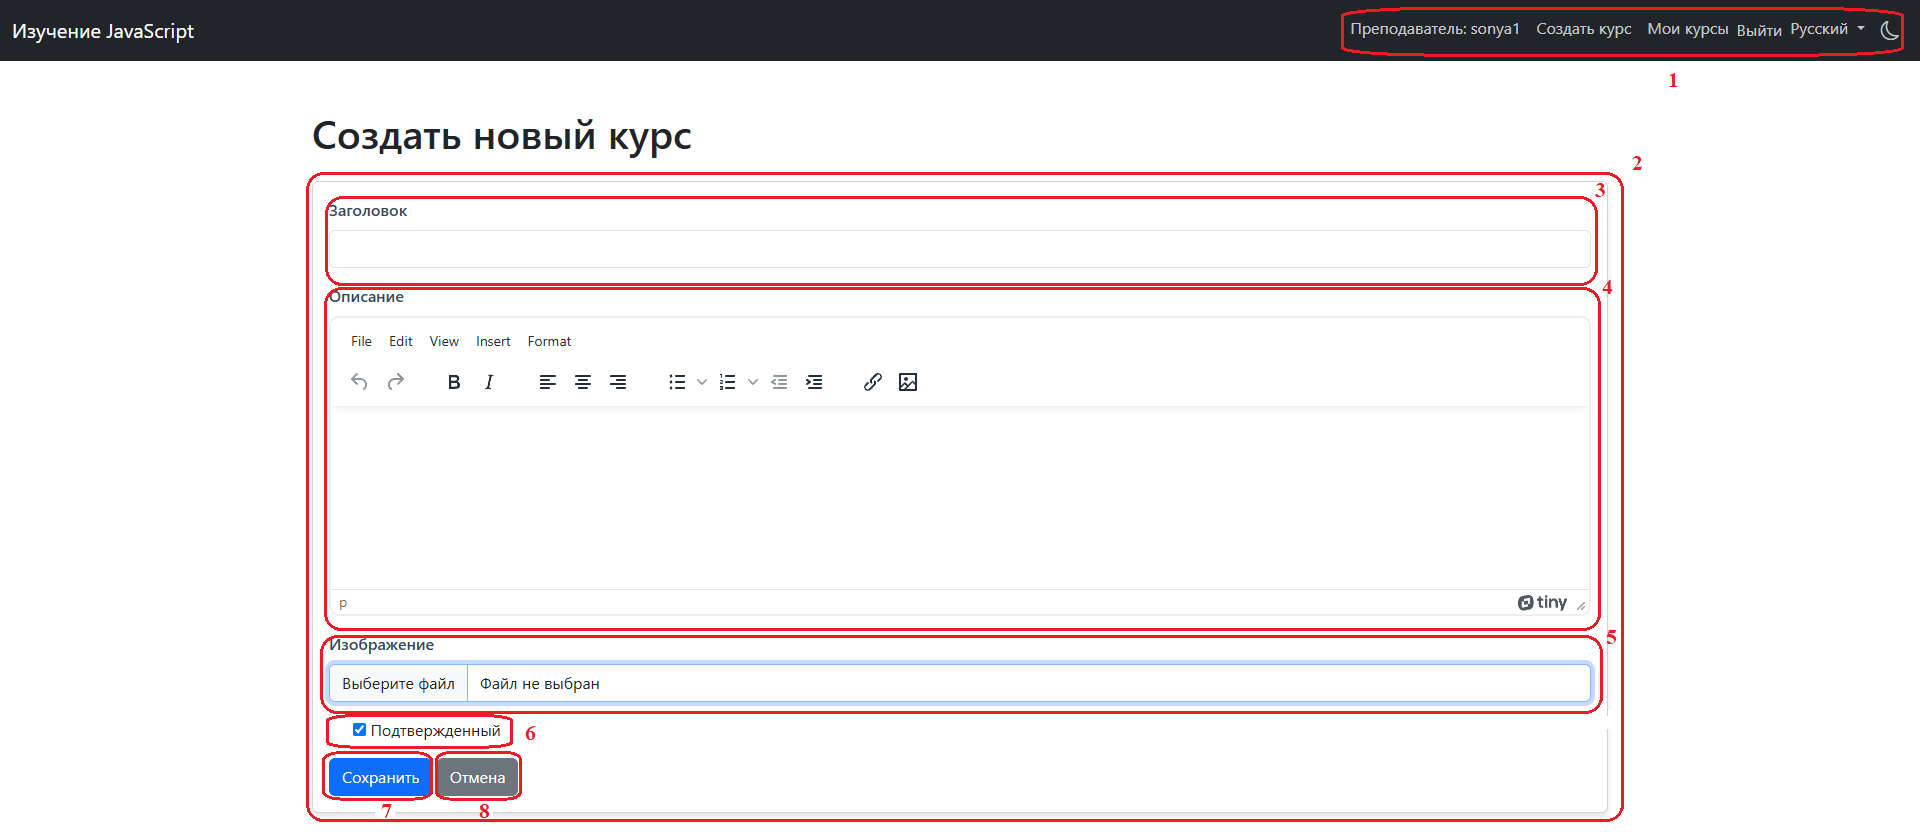
\includegraphics[width=1\linewidth]{images/создатькурс}
	\caption{Композиция интерфейса сервиса <<Создание курса>>}
	\label{templ:image9}
\end{figure}

Композиция шаблона создание урока представлена на рисунке ~\ref{templ:image10} и состоит из:

\begin{itemize}
	\item окно создания урока (1);
	\item поле ввода заголовка урока (2);
	\item поле ввода описания урока (3);
	\item поле ввода материалов урока (4);
	\item поле ввода ссылки на видеоролик (5);
	\item поле выбора статуса урока (6);
	\item кнопка добавления урока (7).
\end{itemize}

\begin{figure}[h]
	\centering
	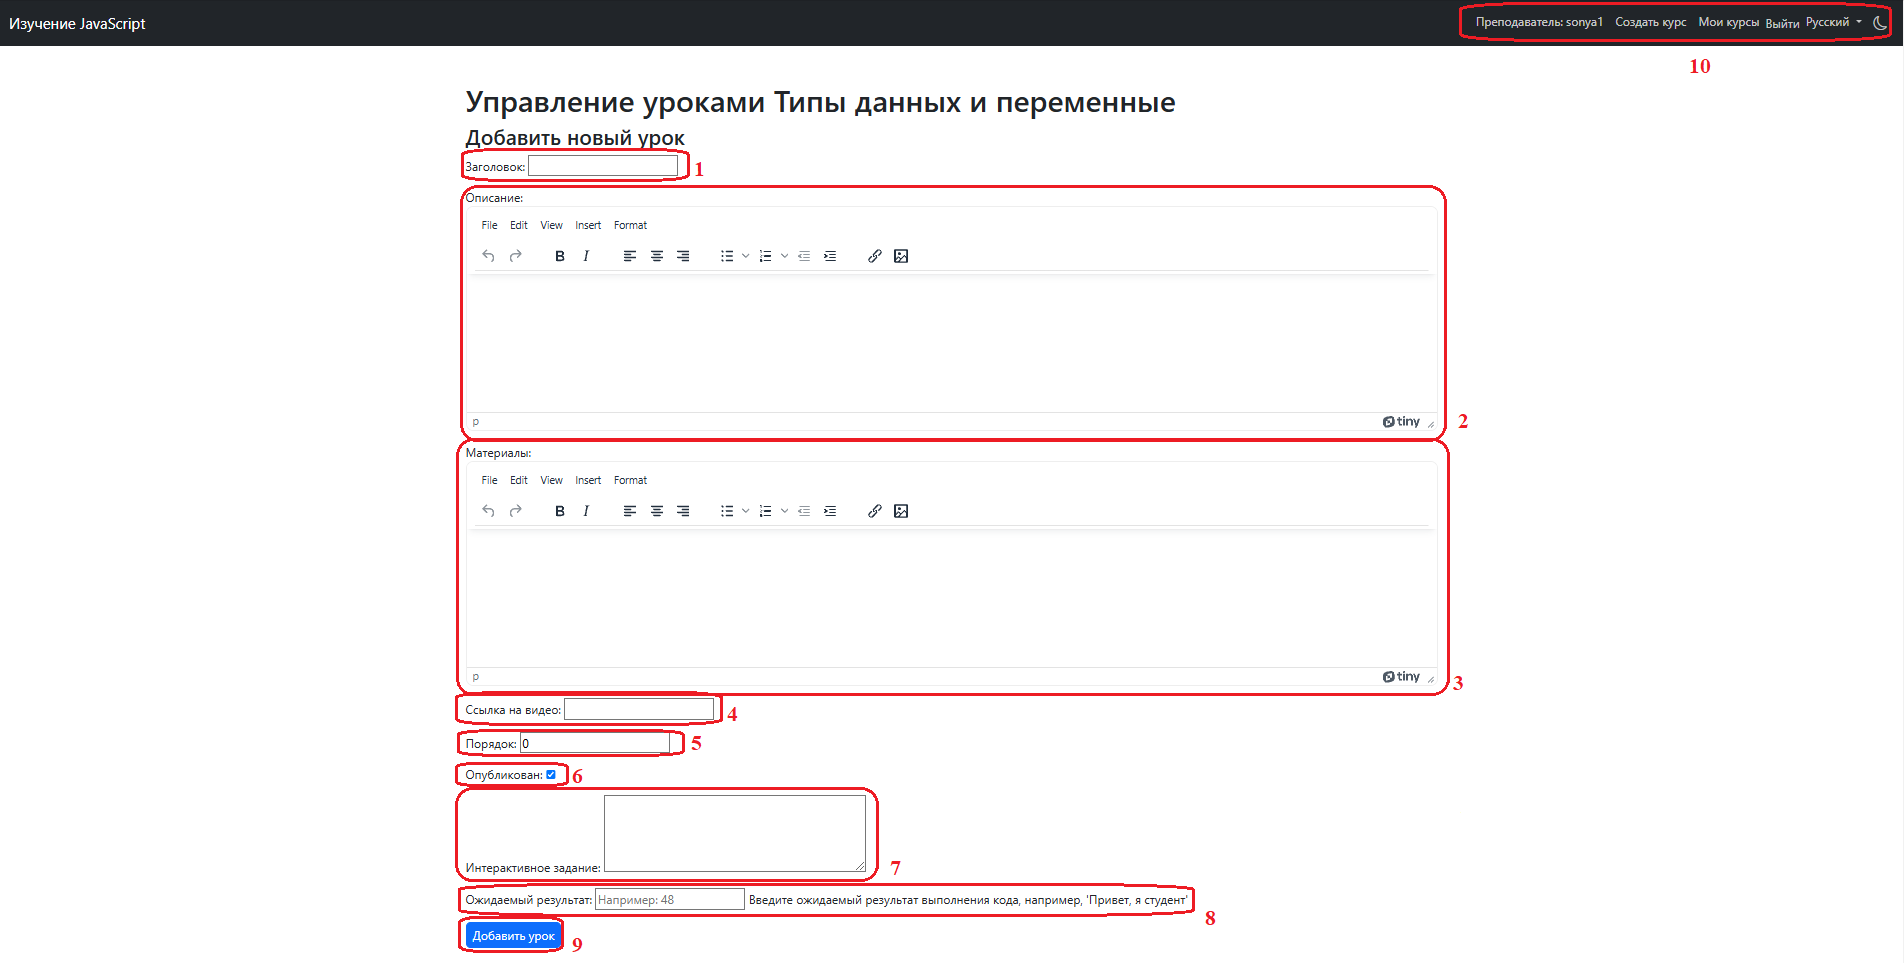
\includegraphics[width=1\linewidth]{images/создатьурок}
	\caption{Композиция интерфейса сервиса <<Создание урока>>}
	\label{templ:image10}
\end{figure}

\clearpage
\subsection{Моделирование вариантов использования}

Для разработки платформы была построена UML-диаграмма вариантов использования, отражающая взаимодействие пользователей с системой.

\begin{figure}[ht]
	\center{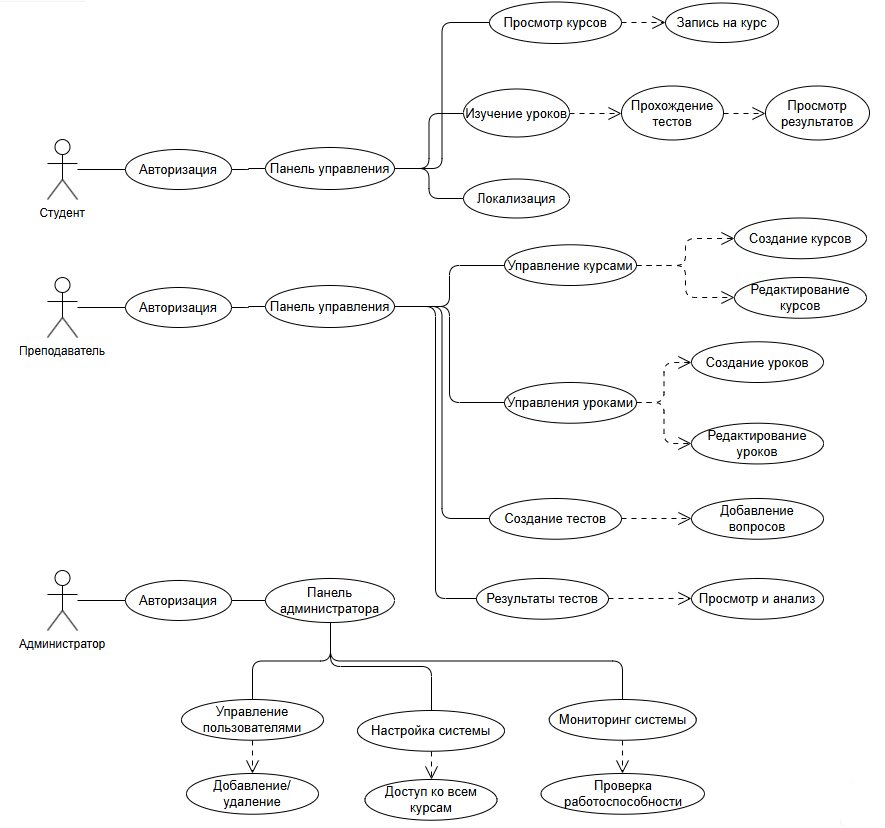
\includegraphics[width=1\linewidth]{images/UML}}
	\caption{Диаграмма прецедентов}
	\label{comp:image}
\end{figure}

Основные прецеденты системы:

\begin{enumerate}
	\item \textbf{Авторизация и выход из системы}: Позволяет пользователям (преподавателям, студентам, администраторам) входить в систему и выходить из неё.
	\item \textbf{Управление курсами}: Обеспечивает создание, редактирование и удаление курсов преподавателями, а также просмотр и запись на курсы студентами.
	\item \textbf{Управление уроками}: Дает возможность преподавателям управлять уроками, а студентам --- изучать их материалы.
	\item \textbf{Создание и управление тестами}: Позволяет преподавателям создавать тесты, а студентам --- проходить их.
	\item \textbf{Прохождение тестов}: Обеспечивает студентам возможность проходить тесты с автоматической оценкой.
	\item \textbf{Просмотр результатов тестов}: Позволяет преподавателям и студентам анализировать результаты.
	\item \textbf{Локализация интерфейса}: Обеспечивает переключение языка интерфейса для удобства пользователей.
\end{enumerate}

После авторизации пользователь переходит на главную страницу: преподаватели видят панель управления, студенты --- список доступных курсов. Ниже приведено подробное описание каждого сервиса и связанных прецедентов.

\begin{enumerate}
	\item \textbf{Сервис <<Курсы>>}
	
	\textbf{Прецедент: Управление курсами (для преподавателей)} \\
	\textit{Цель}: Создание, редактирование и удаление курсов. \\
	\textit{Актёр}: Преподаватель. \\
	\textit{Предусловие}: Преподаватель авторизован и находится в панели управления. \\
	\textit{Основной сценарий}:
	\begin{enumerate}
		\item Преподаватель переходит в раздел <<Курсы>>.
		\item Нажимает кнопку <<Создать курс>>.
		\item Заполняет форму: название (\texttt{title}), описание (\texttt{description}), изображение (\texttt{image}), статус активности (\texttt{isactive}).
		\item Сохраняет курс, система добавляет его в базу данных (\texttt{courses\_course}) и связывает с преподавателем (\texttt{teacherid}).
		\item Для редактирования или удаления преподаватель выбирает курс из списка и выполняет соответствующее действие.
	\end{enumerate}
	\textit{Постусловие}: Курс создан, отредактирован или удалён, изменения отражены в базе данных. \\
	\textit{Альтернативный сценарий}: Если форма заполнена некорректно (например, пустое название), система выдаёт уведомление об ошибке.
	
	\textbf{Прецедент: Просмотр и запись на курсы (для студентов)} \\
	\textit{Цель}: Просмотр доступных курсов и запись на них. \\
	\textit{Актёр}: Студент. \\
	\textit{Предусловие}: Студент авторизован. \\
	\textit{Основной сценарий}:
	\begin{enumerate}
		\item Студент переходит на главную страницу, где отображается список курсов.
		\item Список включает название, описание и статус курса (например, <<Доступен>>, <<Завершён>>).
		\item Студент выбирает курс и нажимает кнопку <<Записаться>>.
		\item Система добавляет запись в таблицу <<Запись на курсы>> (\texttt{courses\_enrollment}) с полями \texttt{courseid}, \texttt{studentid}, \texttt{enrolledat}.
	\end{enumerate}
	\textit{Постусловие}: Студент записан на курс, запись отражена в базе данных.
	
	\item \textbf{Сервис <<Уроки>>}
	
	\textbf{Прецедент: Управление уроками (для преподавателей)} \\
	\textit{Цель}: Добавление, редактирование, сортировка и удаление уроков в рамках курса. \\
	\textit{Актёр}: Преподаватель. \\
	\textit{Предусловие}: Преподаватель авторизован, выбран курс. \\
	\textit{Основной сценарий}:
	\begin{enumerate}
		\item Преподаватель переходит в раздел <<Уроки>> выбранного курса.
		\item Нажимает кнопку <<Добавить урок>>.
		\item Заполняет форму: название (\texttt{title}), описание (\texttt{description}), содержимое (\texttt{content}), ссылка на видео (\texttt{videourl}), порядок (\texttt{order}), статус публикации (\texttt{ispublished}).
		\item Сохраняет урок, система добавляет его в таблицу \texttt{courses\_lesson}.
		\item Для сортировки использует интерфейс с Sortable.js, изменяя поле \texttt{order}.
		\item Для редактирования или удаления выбирает урок из списка.
		\item Может включить предпросмотр урока перед публикацией.
	\end{enumerate}
	\textit{Постусловие}: Урок добавлен, отредактирован, отсортирован или удалён. \\
	\textit{Альтернативный сценарий}: Если видео-URL недействителен, система уведомляет об ошибке.
	
	\textbf{Прецедент: Изучение уроков (для студентов)} \\
	\textit{Цель}: Просмотр материалов урока. \\
	\textit{Актёр}: Студент. \\
	\textit{Предусловие}: Студент записан на курс, урок опубликован. \\
	\textit{Основной сценарий}:
	\begin{enumerate}
		\item Студент выбирает курс и переходит в раздел <<Уроки>>.
		\item Видит список уроков, отсортированных по полю \texttt{order}.
		\item Выбирает урок и просматривает материалы: текст (\texttt{content}), видео (\texttt{videourl}).
		\item После завершения урока система обновляет прогресс (\texttt{courses\_progress}: \texttt{completed}, \texttt{completedat}).
	\end{enumerate}
	\textit{Постусловие}: Урок изучен, прогресс обновлён.
	
	\item \textbf{Сервис <<Тесты>>}
	
	\textbf{Прецедент: Создание и управление тестами (для преподавателей)} \\
	\textit{Цель}: Создание тестов с вопросами и ответами. \\
	\textit{Актёр}: Преподаватель. \\
	\textit{Предусловие}: Преподаватель авторизован, выбран урок. \\
	\textit{Основной сценарий}:
	\begin{enumerate}
		\item Преподаватель переходит в раздел <<Тесты>> урока.
		\item Нажимает кнопку <<Создать тест>>.
		\item Заполняет форму: название (\texttt{title}), описание (\texttt{description}), проходной балл (\texttt{passingscore}), статус (\texttt{isactive}).
		\item Добавляет вопросы (\texttt{courses\_question}): текст (\texttt{text}), тип (\texttt{questiontype}), баллы (\texttt{points}).
		\item Для каждого вопроса добавляет варианты ответа (\texttt{courses\_answer}): текст (\texttt{text}), правильность (\texttt{iscorrect}), порядок (\texttt{order}).
		\item Сохраняет тест, система добавляет его в таблицу \texttt{courses\_test}.
	\end{enumerate}
	\textit{Постусловие}: Тест создан и связан с уроком (\texttt{lessonid}). \\
	\textit{Альтернативный сценарий}: Если проходной балл некорректен, система выдаёт ошибку.
	
	\textbf{Прецедент: Прохождение тестов (для студентов)} \\
	\textit{Цель}: Прохождение теста и получение оценки. \\
	\textit{Актёр}: Студент. \\
	\textit{Предусловие}: Студент записан на курс, тест активен. \\
	\textit{Основной сценарий}:
	\begin{enumerate}
		\item Студент переходит к уроку и выбирает тест.
		\item Система отображает вопросы с вариантами ответов.
		\item Студент выбирает ответы и отправляет тест.
		\item Система автоматически оценивает ответы, сравнивая с \texttt{iscorrect}, и сохраняет результат (\texttt{courses\_testresult}: \texttt{score}, \texttt{answers}, \texttt{attempts}).
	\end{enumerate}
	\textit{Постусловие}: Тест пройден, результат сохранён.
	
	\item \textbf{Сервис <<Результаты тестов>>}
	
	\textbf{Прецедент: Просмотр и анализ результатов (для преподавателей)} \\
	\textit{Цель}: Анализ успеваемости студентов. \\
	\textit{Актёр}: Преподаватель. \\
	\textit{Предусловие}: Преподаватель авторизован, тест пройден хотя бы одним студентом. \\
	\textit{Основной сценарий}:
	\begin{enumerate}
		\item Преподаватель переходит в раздел <<Результаты тестов>>.
		\item Система отображает список студентов, их баллы (\texttt{score}), количество попыток (\texttt{attempts}) и ответы (\texttt{answers}).
		\item Преподаватель может удалить результат, если он некорректен.
	\end{enumerate}
	\textit{Постусловие}: Преподаватель получил статистику по тесту. \\
	\textit{Альтернативный сценарий}: Если результатов нет, отображается сообщение <<Нет данных>>.
	
	\textbf{Прецедент: Просмотр результатов (для студентов)} \\
	\textit{Цель}: Просмотр своих баллов и статистики. \\
	\textit{Актёр}: Студент. \\
	\textit{Предусловие}: Студент прошёл тест. \\
	\textit{Основной сценарий}:
	\begin{enumerate}
		\item Студент переходит в раздел <<Результаты>>.
		\item Система отображает баллы (\texttt{score}), количество попыток (\texttt{attempts}) и правильные/неправильные ответы.
	\end{enumerate}
	\textit{Постусловие}: Студент увидел свои результаты.
	
	\item \textbf{Сервис <<Локализация>>}
	
	\textbf{Прецедент: Локализация интерфейса} \\
	\textit{Цель}: Переключение языка интерфейса. \\
	\textit{Актёр}: Любой пользователь (преподаватель, студент). \\
	\textit{Предусловие}: Пользователь авторизован. \\
	\textit{Основной сценарий}:
	\begin{enumerate}
		\item Пользователь выбирает язык (например, русский или английский) в меню настроек.
		\item Система использует Django i18n для переключения языка интерфейса.
		\item Страница обновляется с новым языком, включая текст интерфейса и вопросы тестов.
	\end{enumerate}
	\textit{Постусловие}: Язык интерфейса изменён. \\
	\textit{Альтернативный сценарий}: Если выбранный язык недоступен, система уведомляет об ошибке.
	
	\item \textbf{Сервис <<Уведомления>>}
	
	\textbf{Прецедент: Получение уведомлений} \\
	\textit{Цель}: Информирование о действиях и ошибках. \\
	\textit{Актёр}: Любой пользователь. \\
	\textit{Предусловие}: Пользователь выполнил действие (например, добавил урок). \\
	\textit{Основной сценарий}:
	\begin{enumerate}
		\item После действия (например, добавления урока) система генерирует уведомление (<<Урок успешно добавлен>>).
		\item Уведомление отображается в интерфейсе (например, в верхней части страницы).
		\item При ошибке (например, некорректный формат данных) отображается сообщение об ошибке.
	\end{enumerate}
	\textit{Постусловие}: Пользователь получил уведомление.
	
	\item \textbf{Сервис <<Панель управления>>}
	
	\textbf{Прецедент: Доступ к панели управления (для преподавателей)} \\
	\textit{Цель}: Быстрый доступ к функциям управления. \\
	\textit{Актёр}: Преподаватель. \\
	\textit{Предусловие}: Преподаватель авторизован. \\
	\textit{Основной сценарий}:
	\begin{enumerate}
		\item После авторизации преподаватель переходит на главную страницу.
		\item Панель управления отображает виджеты: список курсов, уроки, тесты, результаты.
		\item Преподаватель переходит к нужному разделу (например, <<Курсы>>).
	\end{enumerate}
	\textit{Постусловие}: Преподаватель получил доступ к функциям управления.
	
	\textbf{Прецедент: Доступ к списку курсов (для студентов)} \\
	\textit{Цель}: Просмотр доступных курсов. \\
	\textit{Актёр}: Студент. \\
	\textit{Предусловие}: Студент авторизован. \\
	\textit{Основной сценарий}:
	\begin{enumerate}
		\item После авторизации студент переходит на главную страницу.
		\item Система отображает список доступных курсов.
		\item Студент выбирает курс для изучения.
	\end{enumerate}
	\textit{Постусловие}: Студент получил доступ к курсам.
\end{enumerate}

\subsection{Требования к оформлению документации}

Разработка программной документации и программного изделия должна производиться согласно ГОСТ 19.102–77 и ГОСТ 34.601–90. Единая система программной документации.
